\chapter{Metodologia}
\label{chap:metodologia}
	
	Para realização do trabalho proposto adotou-se uma visão macro do projeto no intuito de definir um escopo preliminar, e adequá-lo durante as iterações de tempo fixo de duas semanas. Assim, será possível gerar incrementos constantes no produto até o final do projeto. Para ter uma visão global dos requisitos do produto, adotou-se uma metodologia top/down, investigando a partir de um sistema completo e consistente até o menor bloco hierárquico.

	Uma vez que o tamanho e a complexidade do projeto foram identificados, propôs-se a divisão do trabalho em quatro frentes com projetos menores e distintos, mas complementares, para se chegar a uma solução final coerente com os objetivos esperados. Esta divisão será tratada no subtópico logo a seguir.

	Em relação aos requisitos da solução, no capítulo \ref{chap:desenvolvimento} - \nameref{chap:desenvolvimento} serão especificados os requisitos do projeto de acordo com as perspectivas das subáreas, assim será possível avaliar sobre diferentes aspectos os requistos da solução.

	Para assegurar que todas as partes envolvidas no projeto tivessem o caminho livre de impedimentos para o desenvolvimento de seu trabalho, foi adotado o papel de \textbf{facilitador} \cite{Facilitador}. Ele será responsável por instigar a comunicação, tornando-a horizontal em relação às frentes de trabalho, além de organizar o trabalho gerado e monitorar os resultados esperados ao final de cada iteração. O papel do facilitador será rotacionado ao longo do projeto, sendo definido durante o planejamento da iteração, o qual ocorre no inicio de cada iteração.

	Nas seções a seguir apresentam-se a forma de como o produto será gerenciado ao longo do projeto.


	\section{Organograma}

		Na figura \ref{organograma} apresentam-se os quatro projetos previstos para a divisão do trabalho. Além disso, são indicados os membros por engenharia alocados em cada frente. É importante ressaltar a constante comunicação envolvida em todas as frentes para o sucesso do projeto final.

		\newpage
		\begin{figure}[!h]
			\centering
			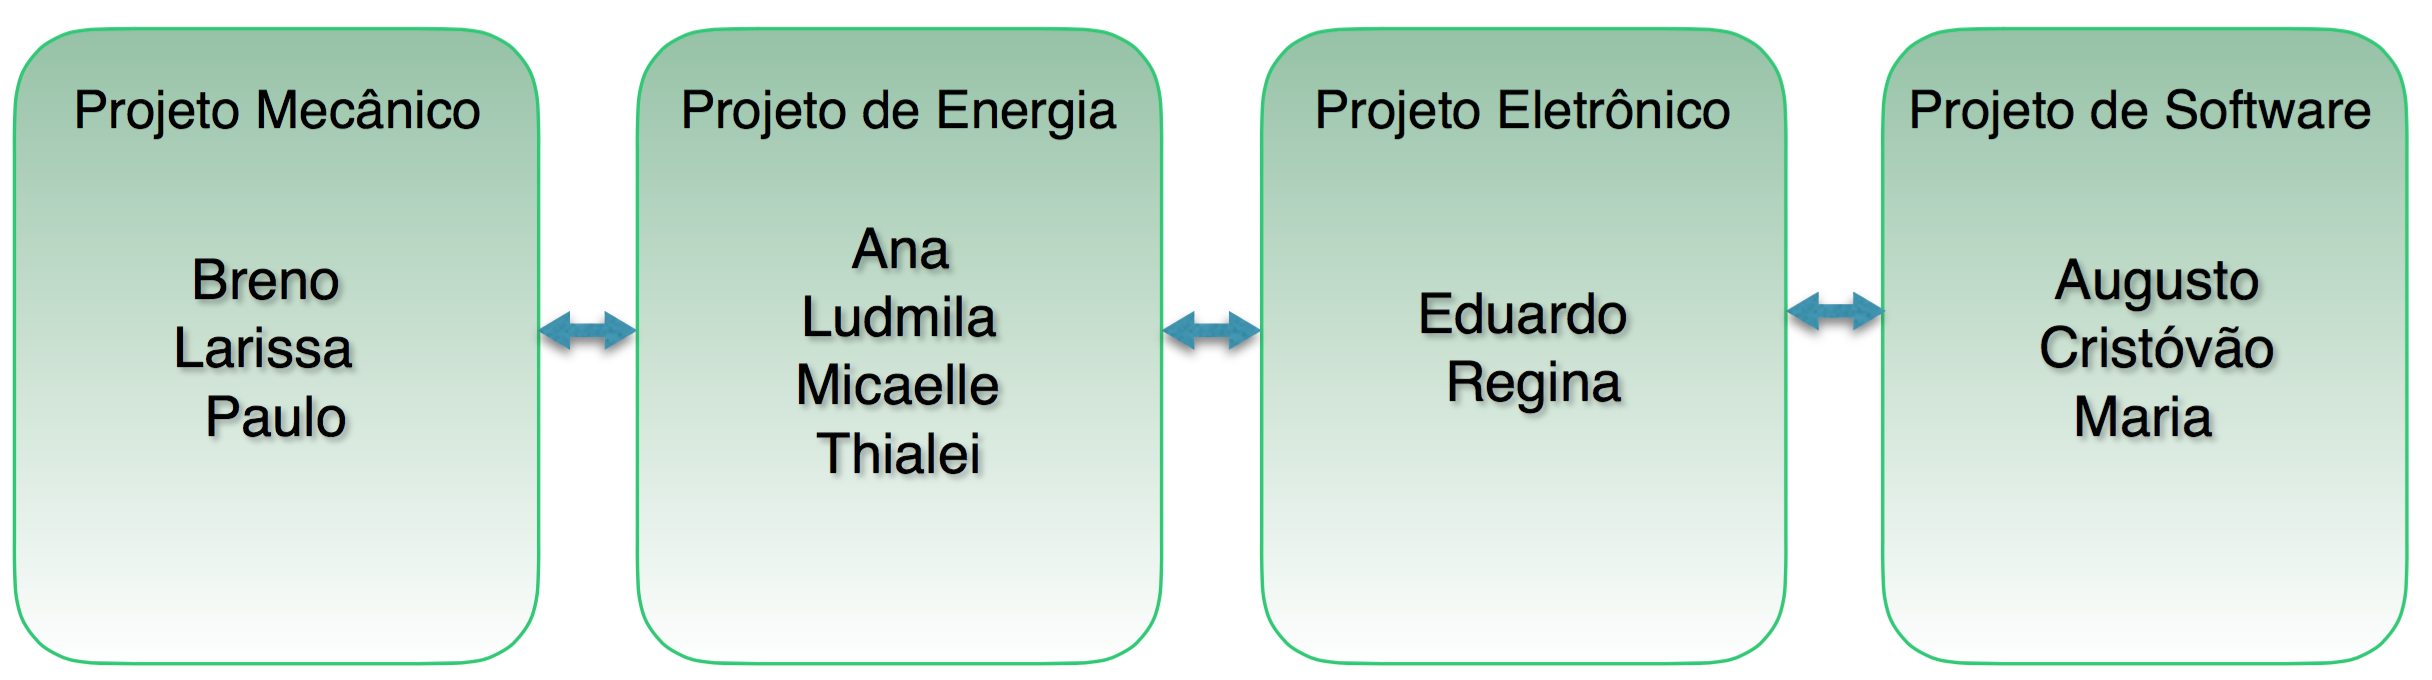
\includegraphics[scale=0.3]{organograma.png}
			\caption{Divisão do trabalho em frente de projetos menores}
			\label{organograma}
		\end{figure}

		No \textbf{Projeto Mecânico} serão tratados todos os componentes físicos da bancada, bem como sua estrutura. Neste projeto deve-se definir as medidas adequadas para a bancada, interconexão dos componentes, robustez da estrutura para o teste e a realização do experimento proporcionando segurança durante sua execução. 
		
		No \textbf{Projeto de Energia} serão compreendidos os aspectos relacionados ao acionamento do motor, controle de velocidades e monitoramento da temperatura do fluido do amortecedor. A partir da definição dos circuitos necessários ao acionamento do motor, ao sistema de proteção e ao controle de velocidade do teste, deve-se fazer as simulações necessárias para garantir o bom funcionamento do sistema.

		No \textbf{Projeto Eletrônico} serão compreendidos os aspectos relacionados à aquisição e processamento de dados, bem como os circuitos eletrônicos necessários para o funcionamento adequado da bancada. Neste projeto deve-se definir todo o tipo de sensoriamento necessário, circuitos de condicionamento, circuitos de proteção contra surtos, simulação dos referidos circuitos e implementação física.

		No \textbf{Projeto de Software} serão tratados os componentes lógicos, ou seja, todos os objetos que o homem controlara por meio do computador. Neste projeto deve-se definir a forma como o experimento será controlado antes, durante e após a execução do experimento e implementar a forma de como os dados serão apresentados aos usuários durante e ao final do experimento.


	\section{Plano de Comunicação}

		As comunicações relevantes para este projeto são definidas na \ref{table_comunicacao}.
		\newpage
		\begin{table}[h]
			\centering
			\caption{Comunicações relevantes para o projeto}
			\label{table_comunicacao}
			\resizebox{\textwidth}{!}{%
			\begin{tabular}{|c|c|c|c|c|}
			\hline
			\rowcolor[HTML]{C0C0C0} 
			\textbf{\begin{tabular}[c]{@{}c@{}}Tipo de\\ Comunicação\end{tabular}} & \textbf{\begin{tabular}[c]{@{}c@{}}Ferramenta /\\ Técnica\end{tabular}} & \textbf{Objetivo} & \textbf{Envolvidos} & \textbf{Frequência} \\ \hline
			\begin{tabular}[c]{@{}c@{}}Reunião para\\ Planejamento da\\ Iteração\end{tabular} & \begin{tabular}[c]{@{}c@{}}Reunião\\ Presencial\end{tabular} & \begin{tabular}[c]{@{}c@{}}Planejar as atividades e resultados da\\ iteração de acordo com o cronograma\\ preliminar\end{tabular} & \begin{tabular}[c]{@{}c@{}}Todos os\\ membros\end{tabular} & \begin{tabular}[c]{@{}c@{}}Inicio de cada\\ Iteração*\end{tabular} \\ \hline
			\begin{tabular}[c]{@{}c@{}}Reunião de\\ Retrospectiva da Iteração\end{tabular} & \begin{tabular}[c]{@{}c@{}}Reunião\\ Presencial\end{tabular} & \begin{tabular}[c]{@{}c@{}}Revisar as lições aprendidas, dificuldades e\\ principais impedimentos para continuidade\\ do projeto\end{tabular} & \begin{tabular}[c]{@{}c@{}}Todos os\\ membros\end{tabular} & \begin{tabular}[c]{@{}c@{}}Fim de cada\\ Iteração*\end{tabular} \\ \hline
			\begin{tabular}[c]{@{}c@{}}Reunião de\\ validação\end{tabular} & \begin{tabular}[c]{@{}c@{}}Reunião\\ Presencial\end{tabular} & Verificar e validar os resultados da iteração & \begin{tabular}[c]{@{}c@{}}Todos os\\ membros\end{tabular} & \begin{tabular}[c]{@{}c@{}}Fim de cada\\ Iteração*\end{tabular} \\ \hline
			\begin{tabular}[c]{@{}c@{}}Avisos e\\ Informativos\end{tabular} & \begin{tabular}[c]{@{}c@{}}Slack /\\ Whatsapp\end{tabular} & \begin{tabular}[c]{@{}c@{}}Divulgar avisos e Informativos aos\\ envolvidos no projeto\end{tabular} & \begin{tabular}[c]{@{}c@{}}Todos os\\ membros\end{tabular} & Semanalmente \\ \hline
			Divulgação de materiais & Drive & \begin{tabular}[c]{@{}c@{}}Armazenar documentos relevantes do\\ projeto\end{tabular} & \begin{tabular}[c]{@{}c@{}}Todos os\\ membros\end{tabular} & \begin{tabular}[c]{@{}c@{}}Quando\\ necessário\end{tabular} \\ \hline
			\end{tabular}%
			}
		\end{table}

		* Iterações terão um tempo fixo de 2 semanas.


	\section{Gerenciamento de Risco}

		O gerenciamento de risco é o processo de identificar, planejar, organizar e controlar todos os recursos envolvidos no projeto no sentido de minimizar os efeitos dos riscos que eles podem influenciar sobre o projeto. Seu principal objetivo é reduzir a probabilidade e impactos dos eventos negativos no projeto, bem como prover orientação das medidas adequadas quando os riscos forem iminentes. 
		
		É importante monitorar e controlar os riscos durante o ciclo de vida do projeto. Para isso, foram definidos escalas de 1 (muito baixo) a 5 (muito alto) indicando a probabilidade e a severidade, ou seja, a classificação do risco conforte apresenta-se na imagem \ref{table_risco_1}.

		\begin{figure}[!h]
			\centering
			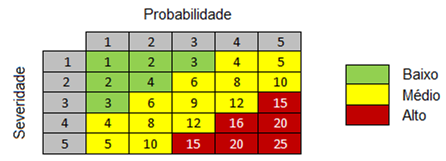
\includegraphics[scale=1]{table_risco_1.png}
			\caption{Matriz de classificação do risco}
			\label{table_risco_1}
		\end{figure}

		Os riscos do projeto são listados na tabela \ref{table_risco_2} a seguir. Nela também é possível visualizar o impacto, sua categoria sendo custo (C) escopo (E) tempo (T) qualidade (Q), a probabilidade de ocorrência, a classificação do risco e a forma de tratamento.

		\newpage
		\begin{table}[]
			\centering
			\caption{Riscos do Projeto}
			\label{table_risco_2}
			\resizebox{\textwidth}{!}{%
			\begin{tabular}{ccccccc}
			\hline
			\rowcolor[HTML]{C0C0C0} 
			{\color[HTML]{000000} \textbf{\begin{tabular}[c]{@{}c@{}}Descrição do\\ Risco\end{tabular}}} & {\color[HTML]{000000} \textbf{\begin{tabular}[c]{@{}c@{}}Categoria\\ do Impacto\end{tabular}}} & {\color[HTML]{000000} \textbf{Consequências}} & {\color[HTML]{000000} \textbf{Probabilidade}} & {\color[HTML]{000000} \textbf{Severidade}} & {\color[HTML]{000000} \textbf{\begin{tabular}[c]{@{}c@{}}Classificação\\ do Risco\end{tabular}}} & {\color[HTML]{000000} \textbf{Ação}} \\ \hline
			{\color[HTML]{000000} \begin{tabular}[c]{@{}c@{}}Inexperiência na\\ gestão do projeto\end{tabular}} & {\color[HTML]{000000} C E T} & {\color[HTML]{000000} \begin{tabular}[c]{@{}c@{}}Atrasos, conflitos\\ internos e prazos\\   inviáveis\end{tabular}} & {\color[HTML]{000000} 4} & {\color[HTML]{000000} 5} & {\color[HTML]{000000} Alto} & {\color[HTML]{000000} \begin{tabular}[c]{@{}c@{}}Consultar e orientadores,\\ estudar gestão de projetos\\   em multidisciplinar.\end{tabular}} \\ \hline
			{\color[HTML]{000000} \begin{tabular}[c]{@{}c@{}}Planejamento\\ inadequado do\\ custo\end{tabular}} & {\color[HTML]{000000} C Q} & {\color[HTML]{000000} \begin{tabular}[c]{@{}c@{}}Prejuízo financeiro\\ para grupo\end{tabular}} & {\color[HTML]{000000} 3} & {\color[HTML]{000000} 5} & {\color[HTML]{000000} Alto} & {\color[HTML]{000000} \begin{tabular}[c]{@{}c@{}}Consultar professores e\\ orientadores.\end{tabular}} \\ \hline
			{\color[HTML]{000000} \begin{tabular}[c]{@{}c@{}}Requisitos mal\\ identificados\end{tabular}} & {\color[HTML]{000000} C T E Q} & {\color[HTML]{000000} \begin{tabular}[c]{@{}c@{}}Tarefas realizadas\\ com má qualidade\end{tabular}} & {\color[HTML]{000000} 4} & {\color[HTML]{000000} 5} & {\color[HTML]{000000} Alto} & {\color[HTML]{000000} \begin{tabular}[c]{@{}c@{}}Consultar referencial\\ teórico, consultar\\   professores.\end{tabular}} \\ \hline
			{\color[HTML]{000000} \begin{tabular}[c]{@{}c@{}}Material não\\ chegar a tempo\\ da entrega\\ do produto\end{tabular}} & {\color[HTML]{000000} C Q} & {\color[HTML]{000000} \begin{tabular}[c]{@{}c@{}}Aumento no custo\\ e diminuição da\\   qualidade do projeto\end{tabular}} & {\color[HTML]{000000} 3} & {\color[HTML]{000000} 5} & {\color[HTML]{000000} Alto} & {\color[HTML]{000000} \begin{tabular}[c]{@{}c@{}}Antecipar a compra dos\\ componentes de acordo\\ com o planejamento.\end{tabular}} \\ \hline
			{\color[HTML]{000000} \begin{tabular}[c]{@{}c@{}}Escopo é identificado\\ como inviável\\ durante a produção\end{tabular}} & {\color[HTML]{000000} C T E Q} & {\color[HTML]{000000} \begin{tabular}[c]{@{}c@{}}Inviabilidade do\\ projeto\end{tabular}} & {\color[HTML]{000000} 3} & {\color[HTML]{000000} 5} & {\color[HTML]{000000} Alto} & {\color[HTML]{000000} \begin{tabular}[c]{@{}c@{}}Redefinir escopo, validar\\ as decisões com os\\   orientadores.\end{tabular}} \\ \hline
			{\color[HTML]{000000} \begin{tabular}[c]{@{}c@{}}Mudanças demasiadas\\ nos requisitos\end{tabular}} & {\color[HTML]{000000} E C} & {\color[HTML]{000000} \begin{tabular}[c]{@{}c@{}}Retrabalho e\\ aumento no custo\end{tabular}} & {\color[HTML]{000000} 2} & {\color[HTML]{000000} 4} & {\color[HTML]{000000} Médio} & {\color[HTML]{000000} \begin{tabular}[c]{@{}c@{}}Refinar escopo com \\ equipes e orientadores.\end{tabular}} \\ \hline
			{\color[HTML]{000000} \begin{tabular}[c]{@{}c@{}}Ausência no\\ comprimento das\\ atividades delegadas\\ aos membros\\ do projeto\end{tabular}} & {\color[HTML]{000000} T C} & {\color[HTML]{000000} \begin{tabular}[c]{@{}c@{}}Aumento no tempo\\ do projeto\end{tabular}} & {\color[HTML]{000000} 2} & {\color[HTML]{000000} 4} & {\color[HTML]{000000} Médio} & {\color[HTML]{000000} \begin{tabular}[c]{@{}c@{}}Alinhar objetivos do\\ trabalho com os objetivos\\   individuais dos membros,\\ e fornecer apoio aos\\ membros quando necessário.\end{tabular}} \\ \hline
			{\color[HTML]{000000} \begin{tabular}[c]{@{}c@{}}Baixa qualidade\\ nos entregáveis\\ do projeto\end{tabular}} & {\color[HTML]{000000} C T Q} & {\color[HTML]{000000} \begin{tabular}[c]{@{}c@{}}Rejeição dos\\ entregáveis pelos\\   avaliadores\end{tabular}} & {\color[HTML]{000000} 2} & {\color[HTML]{000000} 4} & {\color[HTML]{000000} Médio} & {\color[HTML]{000000} \begin{tabular}[c]{@{}c@{}}Refazer os entregáveis\\ e definir margens de\\   qualidade.\end{tabular}} \\ \hline
			{\color[HTML]{000000} \begin{tabular}[c]{@{}c@{}}Atraso no\\ planejamento das\\ atividades\end{tabular}} & {\color[HTML]{000000} C T} & {\color[HTML]{000000} \begin{tabular}[c]{@{}c@{}}Atrasos e aumento\\ do tempo do projeto\end{tabular}} & {\color[HTML]{000000} 2} & {\color[HTML]{000000} 3} & {\color[HTML]{000000} Médio} & {\color[HTML]{000000} \begin{tabular}[c]{@{}c@{}}Reajustar cronograma\\ e aumentar o tempo de\\   trabalho para o período\\ restante.\end{tabular}} \\ \hline
			{\color[HTML]{000000} \begin{tabular}[c]{@{}c@{}}Diminuição da\\ produtividade em\\ semanas de prova\end{tabular}} & {\color[HTML]{000000} C T Q} & {\color[HTML]{000000} \begin{tabular}[c]{@{}c@{}}Diminuição da\\ qualidade nas entregas\\ eaumento do tempo\\ do projeto\end{tabular}} & {\color[HTML]{000000} 1} & {\color[HTML]{000000} 3} & {\color[HTML]{000000} Baixo} & {\color[HTML]{000000} \begin{tabular}[c]{@{}c@{}}Reformar o trabalho\\ nas semanas posteriores\\ a fim de compensar\\ as perdas.\end{tabular}} \\ \hline
			{\color[HTML]{000000} \begin{tabular}[c]{@{}c@{}}Membros desistirem\\ da disciplina\end{tabular}} & {\color[HTML]{000000} T E} & {\color[HTML]{000000} \begin{tabular}[c]{@{}c@{}}Diminuição no escopo\\ do projeto e aumento\\ do tempo de\\ trabalho para\\ outros membros\end{tabular}} & {\color[HTML]{000000} 1} & {\color[HTML]{000000} 3} & {\color[HTML]{000000} Baixo} & {\color[HTML]{000000} \begin{tabular}[c]{@{}c@{}}Informar aos\\ orientadores o quanto\\ antes, e redistribuição\\ das atividades.\end{tabular}} \\ \hline
			{\color[HTML]{000000} \begin{tabular}[c]{@{}c@{}}Artefatos necessários\\ não entregues\end{tabular}} & {\color[HTML]{000000} Q} & {\color[HTML]{000000} Retrabalho} & {\color[HTML]{000000} 1} & {\color[HTML]{000000} 2} & {\color[HTML]{000000} Baixo} & {\color[HTML]{000000} \begin{tabular}[c]{@{}c@{}}Alocar novo membro\\ para realizar a tarefa.\end{tabular}} \\ \hline
			\end{tabular}%
			}
		\end{table}


	\section{Estimativas e Gerenciamento de Custo}

		Os custos são apresentados no capítulo \ref{chap:desenvolvimento} - \nameref{chap:desenvolvimento} de acordo com cada subárea do projeto.
		
		Adicionalmente, para o gerenciamento do custo, foi montado um caixa para o monitoramento de todas as aquisições necessárias ao projeto. Posteriormente o custo total do projeto será dividido entre os membros.